\documentclass{article}
\usepackage{makeidx}
\usepackage[hmargin=3cm, vmargin=2cm]{geometry}
\usepackage{gensymb}
\usepackage{float}
\usepackage{subfig}
\usepackage{graphicx}
\usepackage{rotating}
\usepackage{pstricks}
\usepackage[bookmarks=true, bookmarksnumbered=true]{hyperref}
\pagenumbering{arabic}
\makeindex

\begin{document}
\title{Python Astronomical Stacking Tool Array (PASTA) Manual}
\author{Ben Keller \\ Institute for Space Imaging Science\\
University of Calgary \\ bwkeller@ucalgary.ca}
\maketitle
\begin{center}
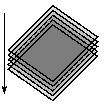
\includegraphics[scale=5]{PASTA_logo.eps}
\vfill
\large{Version 1.0}\\
\normalsize
\date{\today}
\end{center}
\pagebreak
\tableofcontents
\listoffigures
\listoftables
\pagebreak
\section{Introduction}
PASTA is a software package written in the Python programming language for median
stacking of astronomical sources.  It includes a number of features for 
filtering sources, outputting stack statistics, generating Karma annotations, 
formatting sourcelists, and reading information from stacked Flexible Image 
Transport System (FITS) images.  PASTA was originally written to examine 
polarization stack properties, and it includes a Monte Carlo modeller for 
obtaining true polarized intensity from the observed polarization of a stack.  
PASTA is also useful as a generic stacking tool, even if polarization properties
are not being examined.\par

The basic operation of PASTA is to read in a sourcelist containing positions of 
sources to be stacked, as well as one or more FITS images.  PASTA then generates
an output list of stacked sources and their properties, and a pair of FITS 
files, one containing the median pixels of the stack, and the other containing 
the mean pixels.

Stacking allows the reduction of noise levels in the examination of sets of 
images.  It produces a pseudo-source consisting of the median of all the stacked
sources, with reduced background noise level.  For more information on the 
performance of stacking, see \cite[Stil et al. 2010]{stil2010}.

\subsection{Where To Obtain PASTA}
Ask Ben \emph{really} nicely.

\section{Software Requirements}
PASTA uses a number of libraries to be installed prior to running.  Most of these
packages are available in the software repositories of the main Linux 
distributions.

\subsection{Required Packages}
\begin{itemize}
	\item Python $\ge 2.4$ \emph{http://www.python.org}
	\item Numpy $\ge 1.2.0$ \emph{http://numpy.scipy.org}
	\item PyFITS $\ge 2.3$ \emph{http://www.stsci.edu/resources/software\_hardware/pyfits}
	\item Scipy $\ge 0.7.0$ \emph{http://www.scipy.org}
	\item astLib $\ge 0.3.1$ \emph{http://astlib.sourceforge.net}
\end{itemize}

\subsection{Recommended Packages}
The following packages are not needed to run PASTA for stacking, but help for
examining the results and using the plotting utilities.
\begin{itemize}
	\item KARMA \emph{http://www.atnf.csiro.au/computing/software/karma}
	\item matplotlib 0.98.6 or higher \emph{matplotlib.sourceforge.net}
\end{itemize}

\section{Basic Usage}

\subsection{Input Files}
In order to run PASTA, you must first have one or more FITS images and a sourcelist. The sourcelist must be a flat text file, and contain 1 line for each source,
with each column separated by white space. The values for each source must 
include a right ascension, and declination.  You then simply run genstack.py, 
\index{genstack.py} the stack generator, on the sourcelist and images, while 
specifying a stamp size (in pixels). i.e. (for an sourcelist storing the right
ascension in the first column, declination in the second, and the intensity in
the third column):
\begin{center}
\verb!genstack.py -l "0 1 2" source_list source_image.fits 30!
\end{center}
That command will take every source in \verb!source_list! that can be found in 
\verb!source_image.fits! and generate a set of output files, including FITS
images of the median and mean stacked images.

\subsection{Output Files}
After genstack has completed running,  it will create 4 files.  Two of these 
files, \verb!noise_source_list.dat! and \verb!source_list.ann! are flat text 
files.  The former contains a list of values for each stamp.  This file is 
useful for looking at properties of the stack beyond the median/mean intensity,
such as the distribution of background noise, the ratio of accepted/rejected
sources, or for using as a sourcelist for running another stack.
These columns are defined as:
\begin{enumerate}
	\item Right ascension (Degrees)
	\item Declination (Degrees)
	\item Sourcelist intensity (Original list units)
	\item Image intensity (FITS units)
	\item Maximum pixel intensity (FITS units)
	\item X location of maximum pixel
	\item Y location of maximum pixel
	\item Minimum pixel intensity (FITS units)
	\item X location of minimum pixel
	\item Y location of minimum pixel
	\item Absolute Median of outer border (FITS units)
	\item RMS of outer border (FITS units)
	\item Rejection flag 
	\item Source name (Standard IAU format)\\
\end{enumerate} 
The rejection flags are described as follows:
\begin{description}
	\item[a] Stamp accepted for stack
	\item[d] Stamp dimensions do not match specified dimensions, rejected (This
	can occur if the source is closer to the edge of the image than would allow
	a full stamp to be extracted)
	\item[n] Stamp border absolute median above given noise threshold, rejected
	(This occurs when the stamp is pulled from an area of the image with a 
	higher noise than specified.  The absolute median is used to prevent 
	rejection due to interloping sources, and instead only reject on more 
	uniformly high background noise.)
	\item[b] Stamp contains NaN pixels, rejected (This can occur if a source is
	in or near a blank area of the FITS image.)
\end{description}

\begin{sidewaystable}[!htbp]
\begin{tabular}{l | l | l | l | l | l | l | l | l | l | l | l | l | l | l | l}
$\alpha$ & $\delta$ & List Flux & Stack Flux & Max Flux & X & Y & Min Flux & X & Y & Background & RMS Noise & Flag & Name \\
\hline
357.533 & -33.69944 & 2.14000E+00 & 8.16045E-01 & 1.19337E+00 & 22 & 3 & 3.96306E-02 & 11 & 19 & 4.69556E-01 & 5.82890E-01 & a & J235008-331800 \\
1.96625 & 0.71725 & 2.04000E+00 & 6.91129E-01 & 1.72867E+00 & 1 & 6 & 1.86304E-02 & 20 & 21 & 4.22984E-01 & 5.36032E-01 & a & J000751+004300 \\
1.98504 & -0.12561 & 2.14000E+00 & 3.62772E-01 & 2.76332E+00 & 19 & 7 & 4.38120E-02 & 14 & 27 & 5.03270E-01 & 6.14033E-01 & a & J000756-005200 \\
2.05488 & 0.18464 & 2.05000E+00 & 5.54100E-01 & 1.75255E+00 & 8 & 12 & 5.52007E-02 & 28 & 11 & 4.51224E-01 & 6.07346E-01 & a & J000813+001100 \\
2.05758 & -0.18597 & 2.21000E+00 & 1.10080E-00 & 1.62729E+00 & 17 & 15 & 4.46124E-02 & 1 & 18 & 4.69224E-01 & 5.62914E-01 & a & J000813-004800 \\
2.09183 & 0.11883 & 2.06000E+00 & 4.09074E-01 & 1.74689E+00 &  23 &  21 & 2.83552E-02 & 7 & 21 & 4.10038E-01 & 5.08445E-01 & a & J000822+000700 \\
2.13729 & -1.48322 & 2.05000E+00 & 4.24715E-01 & 1.02757E+00 & 4 & 4 & 7.50757E-03 & 12 & 4 & 3.58331E-01 & 4.52300E-01 & a & J000832-013100 \\
2.15954 & -1.52417 & 2.10000E+00 & 1.02308E-01 & 1.08270E+00 & 10 & 2 & 1.70393E-02 & 22 & 10 & 3.19294E-01 & 4.33960E-01 & a & J000838-012800 \\
2.19300 & 0.62006 & 2.03000E+00 & 4.23197E-01 & 1.68701E+00 & 21 & 14 & 4.63659E-02 & 12 & 27 & 6.06562E-01 & 7.57554E-01 & a & J000846+003700 \\
2.23992 & 0.03683 & 2.11000E+00 & 5.23646E-01 & 4.70614E+00 & 20 & 25 & 3.76965E-02 & 1 & 8 & 3.64927E-01 & 7.66693E-01 & a & J000857+000200 \\
\end{tabular}\\
\caption[Example Noise File]{Example Noise File: NRAO VLA Sky Survey (NVSS) Stack, Sources with 2.00-2.24 mJy flux, 30 pixel stamps}
\end{sidewaystable}

\newpage
The second text file contains a set of KARMA annotations that display circles 
over the sources used, and colour codes them.  Accepted sources are green, 
sources rejected due to blank pixels in the stamp are yellow, and sources 
rejected due to high background level are coloured blue. Sources rejected due to
dimension errors are not plotted (as they are dominated by off-image sources).

\begin{figure}[H]
\centering
\includegraphics{annotation.eps}
\caption[Annotation Sample]{Sample of annotation file generated from NVSS stacking (polarized intensity)}
\end{figure}

\pagebreak
The two other files created are both FITS files, 
\verb!source_listsource_image.fits_median.fits! and 
\verb!source_listsource_image.fits_mean.fits! one containing the median pixel 
values of the stack, and one containing the mean pixel values. The following 
example shows a stack with a peak brightness of 2.02 mJy and a root mean square
deviation (RMS) background noise of 0.0465 mJy.  This stack was generated using
a sourcelist and images from the NVSS.\cite[Condon et al. 1998] {NVSS1998} The 
``spokes'' coming from the centre of the source are the sidelobes of the VLA beam.
As these sidelobes lie in the same position within each stamp, they are 
preserved through the stacking process.
\begin{figure}[H]
\centering
\includegraphics[scale=0.75]{stack.eps}
\caption[Stack Sample]{Stokes \emph{I} Stack of NVSS sources from 2.000 to 2.244 mJy, stacked border rms of 46.5 $\mu$Jy}
\end{figure}

\noindent Each of these FITS files contains an additional set of header values. 
These header values contain information about the stack not found in the pixel
data.
\begin{description}
	\item[STACKMIN:] The minimum central pixel intensity in the stack (the 
	0\textsuperscript{th} percentile)
	\item[STACKMAX:] The maximum central pixel intensity in the stack (the 
	100\textsuperscript{th} percentile)
	\item[STACK50:] The median value of the central pixel column in the stacked
	image
	\item[STACK25:] The 25\textsuperscript{th} percentile value of the central 
	pixel column in the	stacked image
	\item[STACK75:] The 75\textsuperscript{th} percentile value of the central 
	pixel column in the	stacked image
	\item[STACKNUM:] The number of stamps used to generate the stack
\end{description}

\section{Features and Options}

\subsection{Genstack Command Line Options}
genstack (The stack generator) includes a number of command line arguments.  
These arguments can be used to control the acceptance of stamps, transformations
done to the individual stamps before stacking, and the what files to output.
\begin{description}
	\item[--help]  Print out a summary of command line options
	\item[-n] The input list is a genstack noise file, use only accepted sources.
	\item[-g n] Regrid by this factor $n$
	\item[-l ``a b c'']  In the input list, the RA, Dec, and intensity are stored in columns $a,b,c$
	\item[-m n] The maximum median background value to accept is $n$
	\item[-s] Save to disk each stamp used in the stack WARNING: Using 
	regridding will cause the astrometry to be incorrect on these saved stamps
	\item[-a] Do not save the annotation file
	\item[-i imagelist] Read in an ASCII file 'imagelist' containing the 
	filenames of the images to be stacked (one file per line). This is
	useful if you have a large number of files to read, and the command line
	can't handle them all.  With this, you don't need 
	\verb!source_image.fits!
	\item[-p n] Also save a FITS file containing the $n$th percentile valued 
	pixels of the stack.
	\item[-d] Similar to the previous option, this option will dump a number of
	stacked images equal to the total number of accepted sources.  These stacks
	all correspond to the total range of percentiles in the stack (in other 
	words, slices from the sorted stack)
	\item[-f ``a b c''] Generate a "fake source" of a simple circular Gaussian 
	centred at the position of the source in the sourcelist, with a peak value 
	of $a$, using the units of the source images, and a Full-Width Half-Maximum		(FWHM) of $b$ pixels.  The peak value is either always $a$ if $c$ is set to
	``d'' (for delta distribution), or a uniform distribution with median $a$ if
	$c$ is set to ``u'' (for uniform distribution).
\end{description}

\subsection{Other Tools}
\subsubsection{readheader.py}
The readheader tool is used to print out the special header values contained in 
the stacked FITS files.  It can either print out a human-readable set of values
and explanations, or print out a single row of data columns for generating 
tables (using the \verb!readheader.py -t! option). All the units on the 
presented data are in the original FITS header units, which will be printed
in the human-readable output along with each value. The columns of this tabular
format is described as follows:

\begin{enumerate}
	\item Minimum Stack Intensity (0\textsuperscript{th} percentile of the 
	stack)
	\item Maximum Stack Intensity (100\textsuperscript{th} percentile of the 
	stack)
	\item Median Stack Intensity
	\item Lowest Quartile Intensity
	\item Highest Quartile Intensity
	\item Border RMS Noise
	\item Border Absolute Median Intensity
	\item Maximum Pixel Intensity
	\item Maximum Pixel X Location
	\item Maximum Pixel Y Location
	\item Minimum Pixel Intensity
	\item Minimum Pixel X Location
	\item Minimum Pixel Y Location
	\item Stamp X dimension
	\item Stamp Y dimension
	\item Number of sources stacked
	\item File name
\end{enumerate}

\subsection{Polarization Estimator Usage}
The polarization estimator tool takes the results of a polarized intensity (PI)
stack along with a Stokes \emph{Q/U} stack and generates an estimate of the 
true median polarization of the stacked sources.  Once a set of these two 
stacks are created, the noise file from the \emph{Q/U} stack is used to start 
the simulator.  Using \verb!Q_noise_file.dat!, the simulator is invoked by:
\begin{center}
\verb!statter.sh Q_noise_file.dat!\\
\end{center}
\par
Once all of the simulation runs are complete, you can obtain the most likely 
true polarization by finding the resulting true polarization (as indicated
in the output file name) whose file has a median polarization value closest to 
the stack observed polarization.

\section{Internal Operation}

\subsection{Stack Generation}

\subsubsection{Stamp Creation}
Once a sourcelist and FITS files have been read by genstack.py, the program 
proceeds to extract ``stamps'', square sections of the source image with a 
source centred within them.  Each of these stamps has a number of calculations 
performed on it.  If the regridding option has been selected, the image 
resolution is increased by the specified factor using cubic spline 
interpolation.  The stamp is then shifted to centre the source more 
accurately, and it is then regridded back to the original resolution. The 
brightest and dimmest pixel locations are then found, and the pixel coordinates
within the stamp are recorded. \par

A border region is then calculated.  This border is simply all the pixels in 
the image within a threshold value from the edge of the stamp. This thickness 
threshold is the greater of either 5 pixels or 20 percent of the length of a 
stamp side. Of the pixels in this border region, and RMS values are 
calculated and stored, along with the median of the absolute value of each 
pixel. The median absolute value $\hat\sigma$ is used as a robust estimator of 
the RMS.  $\hat\sigma$ is somewhat less affected by nearby sources, as well as 
able to work with Stokes \emph{Q/U/V} images, in which negative intensities can occur without introducing any ambiguity.  This absolute median can be used to 
calculate the rms.  For a Gaussian distribution, the absolute median 
covers 50\% of the distribution.  This same amount of area is covered by 
$0.67443\sigma$, and therefore
$$\sigma \approx \hat\sigma/0.674443$$
\par

After these calculations complete, each source is assigned conditional flags.
The first check is simply to ensure that the stamp has the same dimensions as
specified by the size option (stamps from the borders of images may contain only
a portion of a full stamp.) If the absolute median is found to be above 
the maximum specified noise (default value is infinite), a stamp will be 
rejected as too noisy.  If this flag is not tripped, but the raw RMS of the 
border is above the maximum specified noise, this is flagged as having a 
possible interloping source, but still used in the stack.  The final check is to
ensure that the stamp does not contain any blank or NaN pixels, as these 
interfere with the statistics of the final stacked results (by giving some
pixel columns more sources to stack than others).\par

If the ``save stamps'' option has been selected, the stamp will then be written 
out to a specific fits file.  This feature can be useful for creating individual
source images of a list of sources, as well as stacking.

\subsubsection{Regridding}
If regridding is specified in the command-line arguments, before each stamp
is finally added to the stack, PASTA will interpolate the image up by the factor
specified in the arguments. The interpolation scheme is a simple two-dimensional
cubic spline.  Once this is complete, the image is shifted to move the source 
centre (as found in the source list) to the centre of the higher resolution 
image.  This shifting is done using Numpy's \verb!numpy.roll()! method, and the
interpolation uses \verb!ndimage.zoom()!. The stamps initially generated with 
the regridding option enabled have dimensions of $\mathrm{(N+2)x(N+2)}$ for a 
stamp size of N. This allows PASTA to trim the extra border of pixels off the 
image after it is regridded, in order to prevent edge-located objects and 
structure from tearing when the image is shifted.   Once the image is then 
interpolated and shifted, the image is interpolated down to the original 
dimensions, and the extra pixels are trimmed off, resulting in a $\mathrm{NxN}$
stamp with a more accurately centred source.

\subsubsection{Seeding Fake Sources}
If the user requests a fake source to be seeded, and specifies a peak and FWHM 
value for the simulated sources, the following process will be applied to each 
stamp.  After regridding is completed, a value will be drawn from a uniform 
distribution between 0 and twice the peak value (thus having a median value of
the specified peak) if the uniform distribution is set. If the delta 
distribution is set, the peak value is simply set to the input peak value.
A 2D, circular Gaussian with a FWHM (in pixels) as 
specified by the user is then generated with 
\verb!Numpy's ndimage.filters.gaussian\_filter()! method.  The peak is then 
scaled to match the random value previously drawn.  This is then added to the 
stamp, and the stacking process resumes as usual.

\begin{figure}[H]
\centering
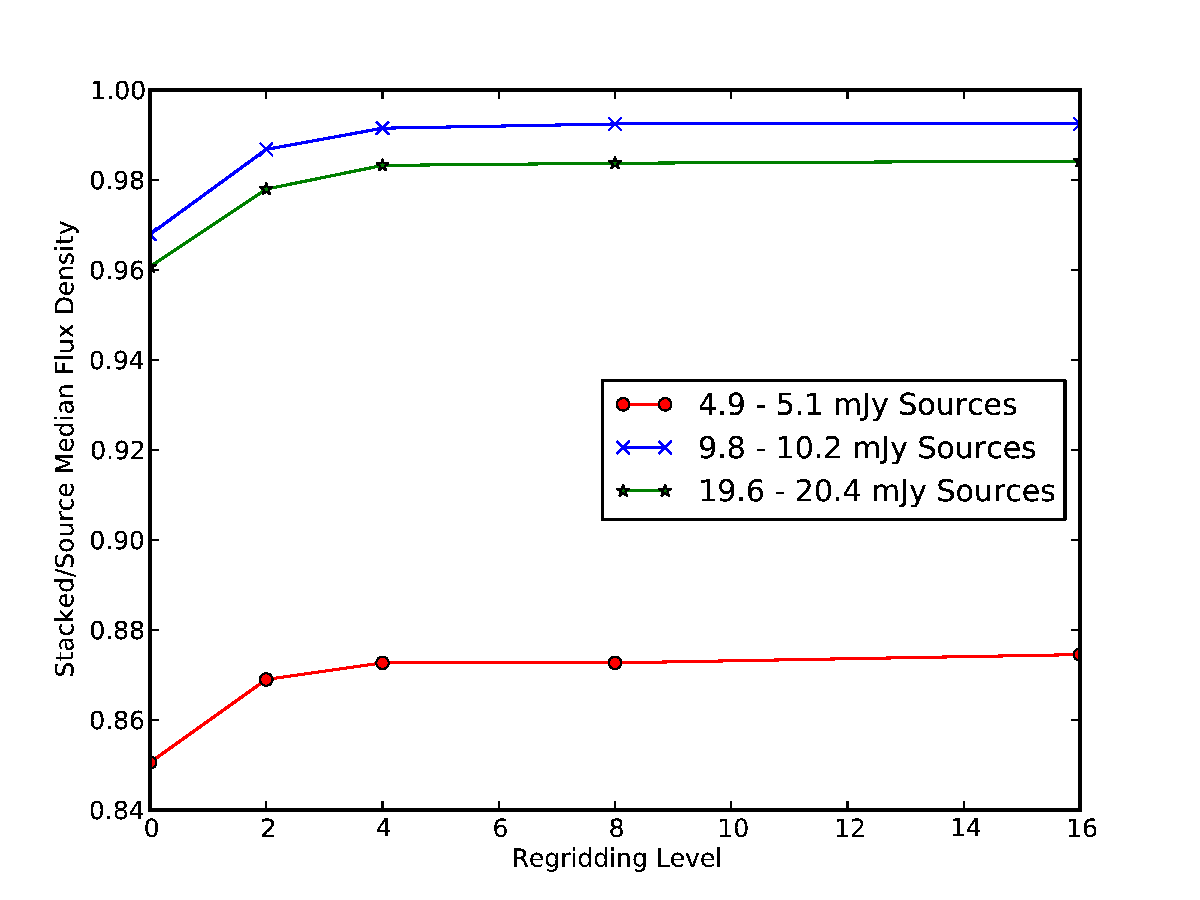
\includegraphics[trim=0cm 0cm 0cm 0cm, clip, scale=0.7]{regridding.eps}\\
\caption[Regridding Performance Increase]{Accuracy of stack results as a 
function of the regridding level (shown for three different flux levels)}
\end{figure}


\subsubsection{Stack Creation}
As the stamps are created, if they are found to have no error flags, they are
added to the stack.  This stack is simply a 3-dimensional matrix of 
intensity values, with the first two dimensions (the stamp dimensions) holding 
spatial information.  Once the stack has been fully populated with stamps, two 
2-dimensional matrices are generated.  These are the median and mean 
output images, and are generated by taking the mean and median, respectively, 
along the third dimension of the stack.  These values are calculated using 
Numpy's \verb!numpy.median()! and \verb!numpy.average()! methods. Each of these
is written out as its own FITS file, with the additional header values specified
previously.  The 25\textsuperscript{th} and 75\textsuperscript{th} percentile 
header values of the central pixels are also calculated along the third 
dimension.  Along with these FITS files, the annotation and noise tables 
created using data from each stamp are written out.

\subsection{Polarization Estimator}
The results of a polarized intensity stack cannot be taken at face value to represent the true polarized intensity the result, as it has been long known that
polarized observations are subject to bias.  Removing this bias has been 
discussed heavily in the past, and the general distribution of polarized sources
has been found to be Ricean \cite[Simmons \& Stewart 1985]{SandS1985}.  In order
to take the results of a polarized intensity stack and obtain an estimate for 
the true polarized intensity of that stacked image, a Monte Carlo tool for 
estimating true polarized intensity has been provided.

\subsubsection{Monte Carlo Modeller}
To obtain a value for true polarization from an observed polarization an 
estimate of the percentage for the observed flux due to noise in the image must
be determined.  The best way to determine this is to find a distribution of the
noise, and run Monte Carlo analysis with different intensities to find the most
likely true polarized intensity which yields the observed polarization in the
stack.\par
For a given true polarized intensity, the modeller draws a value from a 
polarized intensity distribution, and scales this value by the true 
polarization.  It then takes a given Q/U absolute median, and draws a value from
a noise distribution, scaling this value by the given noise value.  It then uses
this to generate an observed polarization value.  For each stamp in a Q/U stack,
the noise is read from the noise file generated by the stacker and run through
the modeller.  The median of the resulting observed polarization values is taken
to create a simulated median stack.\par

This process is repeated 5000 times, and the true polarization found to be the 
value that produces a median polarization closest to the result of the 
polarization stack.  Error estimates are produced by calculating the 
16.5\textsuperscript{th} and 83.5\textsuperscript{th} percentile values that 
best fit the observed polarization (2/3\textsuperscript{rds} of the expected values should lie within this range).

\subsubsection{Polarization Distribution}
In order to approximate the Rice distribution of polarized sources, an
approximated distribution based on the \cite[Beck \& Gaensler 2004]{BandG2004}
distribution is used.

\subsubsection{Noise Distribution}
The included noise distribution used with the modellers was determined 
empirically from the NVSS survey images.  By masking out sources, the background
of the image was determined, and then a distribution consisting of the sum of a
Gaussian and exponential \cite[Stil et. al 2010]{stil2010} was fit to the 
resulting intensity distribution.  As the noise levels, as well as 
artifacts/systematics, of different survey images will be different, this 
likely will need to be re-done for each different image survey set used.

\section{Stack Performance}
The noise level of a stacked image composed of N stamps, with initial RMS noise of $\sigma_0$ is roughly 
$$ \sigma = \frac{\sigma_0}{\sqrt{N}}$$
The actual performance is shown to conform well to this expected rate in 
polarized intensity, as shown in Figure 3.
\begin{figure}[H]
\centering
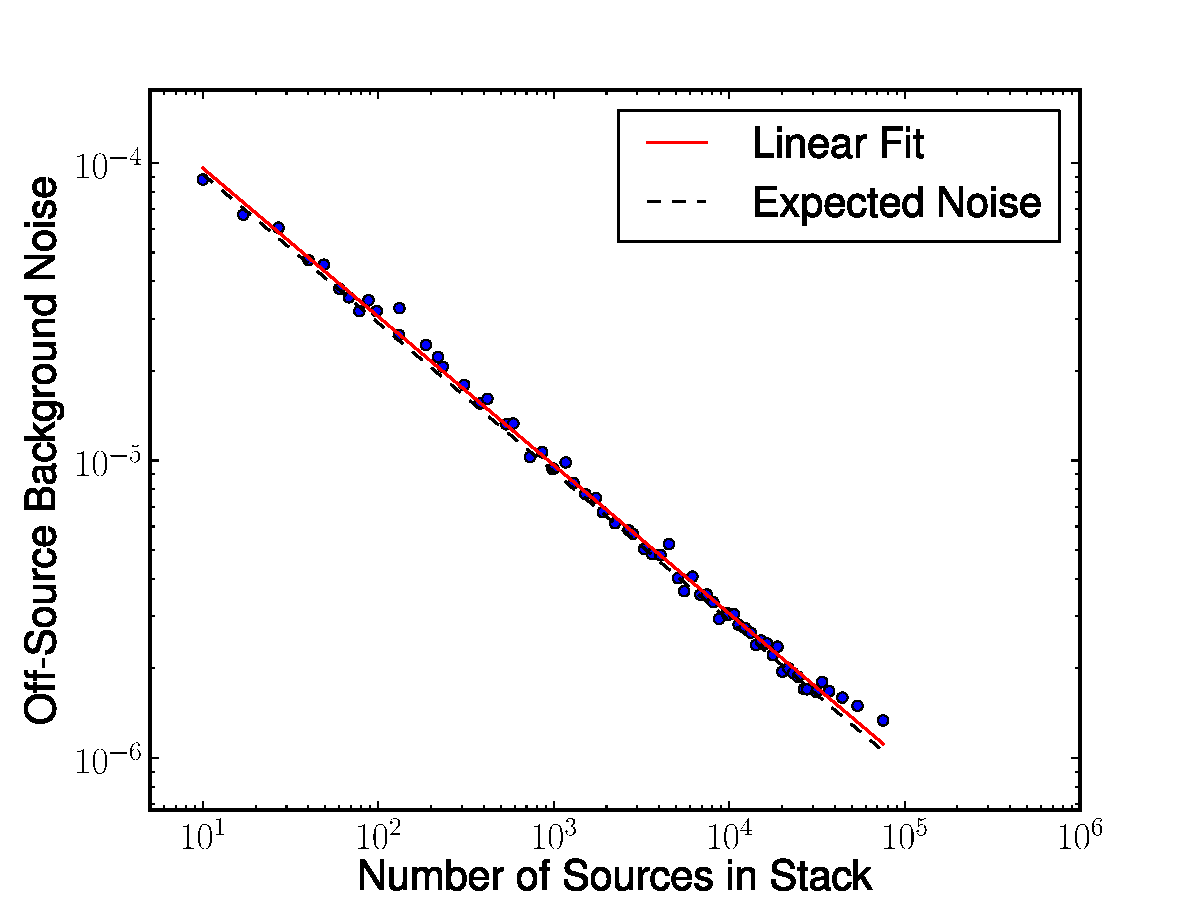
\includegraphics[trim=0cm 0cm 0cm 0cm, clip, scale=0.7]{Noise_vs_Num.eps}\\
\caption[Stacking Performance for NVSS PI]{Background rms versus number of 
sources stacked (in polarized intensity)}
\end{figure}
The slope of the fitted line was found to be -0.49889, a 0.022\% error from the expected -0.5, and the intercept was found to be -3.51871.  This corresponds
to a $\sigma_0$ of 0.303 mJy, while the NVSS images used had a $\sigma_0$ of 
0.29 mJy \cite[Condon et al. 1998]{NVSS1998}, an error of 4.4\%.  The RMS of 
this error value was found to be 5.7\% of the total RMS.\par

Similar performance can be found in the FIRST, VLSS, and NVSS Stokes I 
when random positions are stacked.  We stacked random positions in order to 
prevent the increase in noise due to the sidelobes of the beam used to observe
the objects.  This noise increase can be seen by comparing the relatively low 
brightness Principal Galaxy Catalogue (PGC) objects stacked in similar numbers: at
low enough noise, the flux from the sidelobes decrease the performance of the 
stack.  If the stacked image was CLEANED, or if the beam was weighted out of the
noise calculations, similar performance to the theoretical $\sqrt{N}$ noise 
reduction can likely be obtained.
\begin{figure}[H]
\centering
\includegraphics[trim=0cm 0cm 0cm 1cm, clip, scale=0.7]{VLSS_noise_vs_num.eps}\\
\caption[Stacking Performance for VLSS]{Background rms versus number of 
sources stacked, random sources and PGC galaxies (VLSS images)}
\end{figure}

\begin{figure}[H]
\centering
\includegraphics[trim=0cm 0cm 0cm 1cm, clip, scale=0.7]{NVSS_noise_vs_num.eps}\\
\caption[Stacking Performance for NVSS I]{Background rms versus number of 
sources stacked, random sources and PGC galaxies (NVSS images)}
\end{figure}

\begin{figure}[H]
\centering
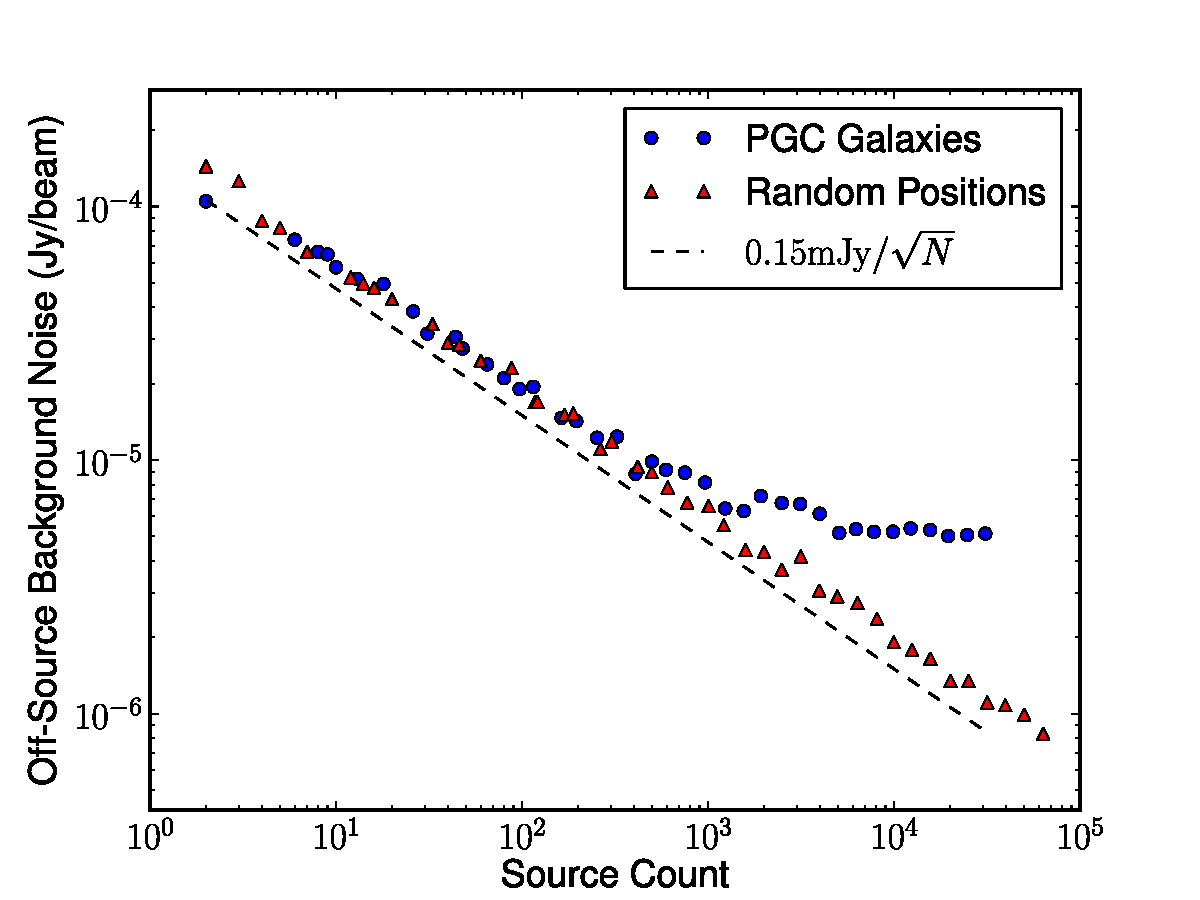
\includegraphics[trim=0cm 0cm 0cm 1cm, clip, scale=0.7]{FIRST_noise_vs_num.eps}\\
\caption[Stacking Performance for FIRST]{Background rms versus number of 
sources stacked, random sources and PGC galaxies (FIRST images)}
\end{figure}
\subsection{Limitations}
\subsubsection{Positional Accuracy}
Because PASTA relies on the ability to place sources in an overlapping stack 
centred on each source's peak, the accuracy of positions given in the sourcelist
is extremely important.  Inaugurate positions cause flux to ``leak'' into 
adjacent pixels to the central pixels, causing the peak flux to be lower than 
the true median of the sources, and creating a larger source than should be 
found.  This issue is why we regrid sources before stacking them, to ensure that
sub-pixel resolution positions are used (images stacked without regridding 
exhibit the same limitations as images stacked with less accurate positions)\par

The effects of positional accuracy can be shown in the comparison of a sample of
sources stacked using positions from the NVSS and the Faint Images of the Radio
Sky at Twenty Centimetres (FIRST) survey.  Both surveys were made with the VLA, 
but the FIRST used the VLA B configuration, with a synthesized beam of roughly 
5'', where the NVSS was observed using the VLA D configuration, with a beam of 
45''.  Thus, the FIRST source positions are expected to be more accurate than 
the positions in the NVSS catalogue, with an expected positional error 
$\approx1/9$\textsuperscript{th} the magnitude of the NVSS.  A subset of sources
found in both the NVSS and FIRST was selected with a NVSS peak intensity of 
between 3 and 5 mJy, and then stacked using both the NVSS positions and the 
FIRST positions for both the NVSS and FIRST images. The differences in flux and source size are not as obvious in the stacks derived from NVSS images, but in 
the stacks generated from the FIRST images, the source is clearly ``blurred''. 
The blurred stack shows a larger apparent source, with a lower peak intensity. 

Fitting of source sizes is a simple test one can run on the results of a stack.
This can be used as a test of both the positional accuracy, as was shown in 
comparing the NVSS and FIRST positions, and in testing that the sources stacked
are indeed unresolved.  If stacked image produces a source the same size of the
beam, this will confirm that the positional accuracy is sufficient, and that
the stack is dominated by unresolved sources.

\begin{figure}[H]
\centering
\subfloat[NVSS positions]{\includegraphics[trim=0cm 6cm 0cm 7cm, scale=0.4]{NVSSposNVSS.eps}}
\subfloat[FIRST positions]{\includegraphics[trim=0cm 6cm 0cm 7cm, scale=0.4]{FIRSTposNVSS.eps}}
\caption[NVSS image position comparison]{NVSS images stacked using FIRST and 
NVSS positions }
\end{figure}

\begin{figure}[H]
\centering
\subfloat[NVSS positions]{\includegraphics[trim=0cm 7.2cm 0cm 7cm, scale=0.4]{NVSSposFIRST.eps}}
\subfloat[FIRST positions]{\includegraphics[scale=0.4]{FIRSTposFIRST.eps}}
\caption[FIRST image position comparison]{FIRST images stacked using FIRST and 
NVSS positions }
\end{figure}
\subsubsection{Unresolved Structure \& Directionality}
For objects such as spiral galaxies, two similar unresolved sources can have 
significantly different flux due to unresolved properties.  One such example
is the axial ratio of spiral galaxies ($B_{maj}/B_{min}$), ie. face-on versus 
edge-on orientation.  A face-on galaxy will obviously have a larger solid angle 
than an edge-on galaxy at the same distance.  This will affect the flux observed
from that galaxy.  This effect can be observed by stacking lists of similar 
galaxies split into bins by their axial ratio.  The following stacks and plots
were generated by doing this to a list of spiral galaxies obtained from 
the PGC type Sb and Sc spiral galaxies, using NVSS Stokes I images.  The peak
flux density obtained from stacking these galaxies altogether, with axial ratio
below 1.3 (face on), and above 4.0 (edge on), were 727.03 $\mu$Jy, 1.04 mJy, and
430.06 $\mu$Jy respectively.

\begin{figure}[H]
\centering
\includegraphics[scale=0.5]{spirals.eps}
\caption[Stacked spiral galaxies without axial ratio split]{Stack of spiral 
galaxies without selection by axial ratio}
\end{figure}

\begin{figure}[H]
\centering
\subfloat[Axial Ratio below 1.3 (face on)]{\includegraphics[scale=0.4]{spirals_ratio_low.eps}}
\subfloat[Axial Ratio above 4.0 (edge on)]{\includegraphics[scale=0.4]{spirals_ratio_high.eps}}
\caption[Stacked spiral galaxies with axial ratio split]{Stacks of spiral 
galaxies with axial ratio below 1.3 and above 4.0}

\end{figure}
\begin{figure}[H]
\centering
\includegraphics[scale=0.8]{spiral_axial_ratio.eps}
\caption[Plot of Flux vs. Axial Ratio for spiral galaxies]{Median Stokes I flux
as a function of axial ratio $B_{maj}/B_{min}$ in spiral galaxies}
\end{figure}
%\subsubsection{Numerical Precision}
%TODO
\section{Usage Example: Simulation Stacking}

\subsection{Introduction}
In order to test the behaviour of the modeller and the stacking process in 
comparison to known results.  In order to do this, a set of simulated images
were seeded with sources of a known percentage polarization, and stacked.  This
allowed us to verify that the true polarization produced by the stacking and
modelling matched the polarization of the simulated images.

\subsection{Simulated Image Generation}
The simulated images are intended to match as closely as possible the images 
of the real NVSS.  The steps used to generate these images are as follows:
\begin{enumerate}
	\item Each $4\degree$ by $4\degree$ simulated image is first seeded with 
	1639 sources, the average number of polarized sources found in a real NVSS 
	tile. These sources have random intensity with a median polarized intensity 
	constant across brightness at ~2\% of the total source brightness.  These
	sources are seeded using the same beam produced by the Very Large Array (VLA) antenna 
	configuration in the NVSS
	\item Once all 1639 sources have been seeded, Gaussian noise is added to 
	each image, along with a random weighting to simulate areas of poor 
	coverage in our real NVSS images.
	\item The images are used to create FITS files of PI, as well as Stokes 
	\emph{I,Q,U}, and the source information is written out into a sourcelist 
	for this set of images.
	\item This process is repeated 479 times to produce an area covering a band
	about the celestial equator from -20\degree to 20\degree declination.
\end{enumerate}
\pagebreak
\begin{figure}[H]
\begin{center}
\includegraphics[trim=0cm 0cm 0cm 0cm, clip, scale=0.65]{Simulation_I.eps}\\
\end{center}
\caption[Simulated NVSS Stokes I image]{Simulated NVSS Stokes I $4\degree$ by 
$4\degree$ image tile}
\end{figure}
\begin{figure}[H]
\begin{center}
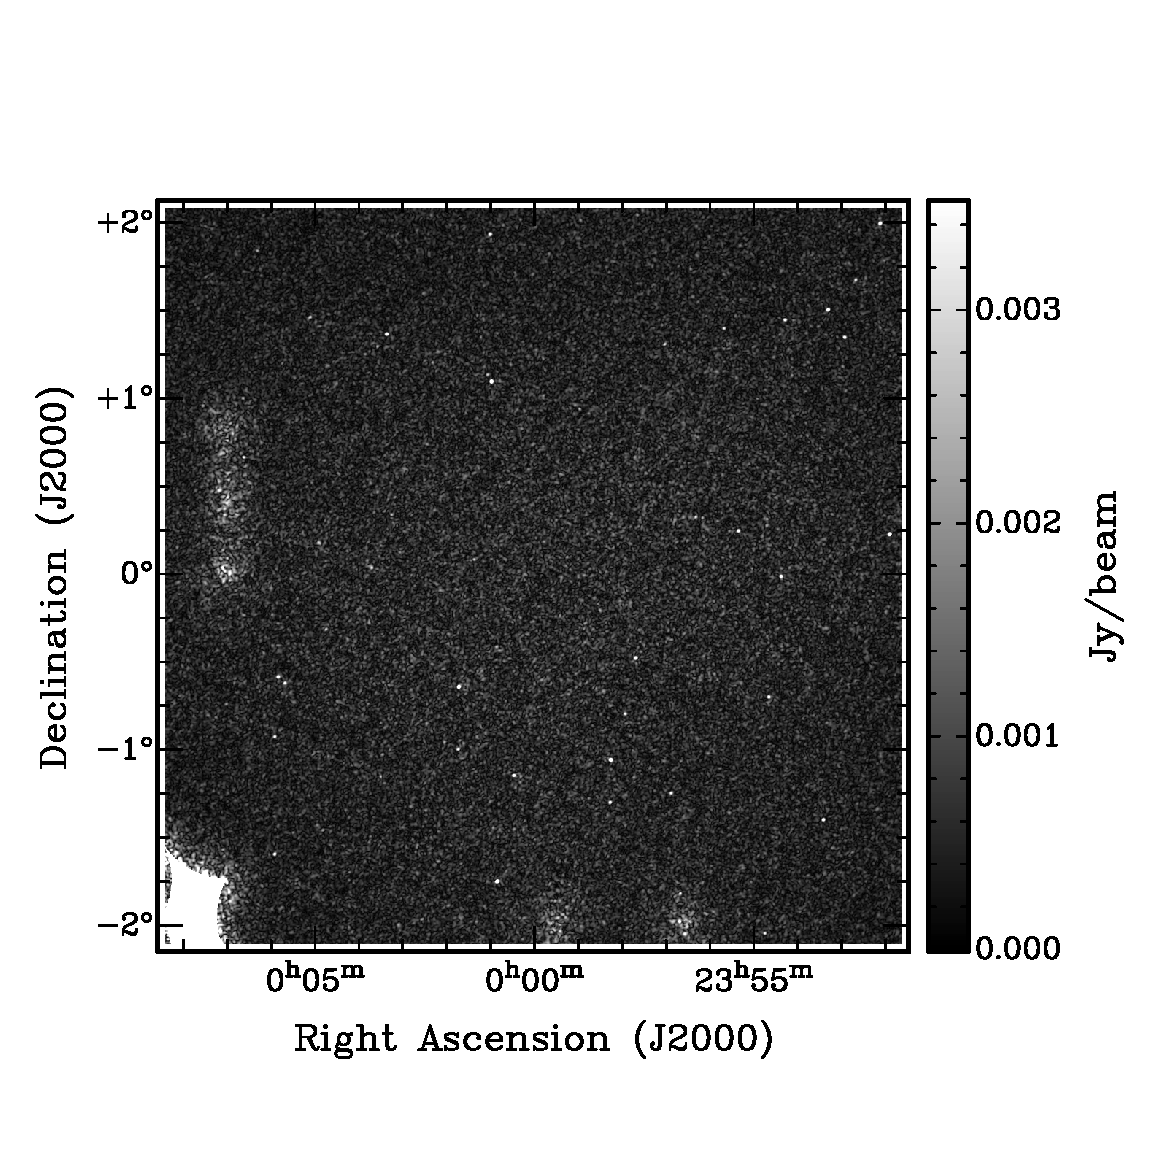
\includegraphics[trim=0cm 1cm 0cm 1cm, clip, scale=0.65]{Simulation_PI.eps}\\
\end{center}
\caption[Simulated NVSS PI image]{Simulated NVSS Polarized Intensity 
$4\degree$ by $4\degree$ image tile}
\end{figure}

\subsection{Stacking the Simulation}
The process of stacking the simulated images is essentially the same as the 
process for stacking the real NVSS images.  Obviously, the only difference is 
that the sourcelists and images are the simulated images and the sourcelist for
the simulated sources. \par

The modeller was running using the same PI distribution as the NVSS, with 
a similar Gaussian plus exponential distribution for the noise.  The noise 
distribution used slightly different parameters that were obtained empirically 
from the images using the same technique as the one used to generate the noise
distribution parameters for the NVSS images.

\subsection{Analyzing the results}
As the figure on the next page shows, the simulation images have similar 
properties to the real NVSS images when stacked.  In the bottom pane showing
the percentage polarization, it is clear that from ~1 mJy to ~500 mJy Stokes
\emph{I} intensity, the percentage polarization remains fairly constant, 
consistent with the seeded polarization.\par

In the high intensity end of the curve, we find the percentage polarization 
diverging above the constant value, as does the low intensity end.  Both of 
these regions are expected to have less reliable polarization estimates.  The 
higher intensity region suffers from lower source counts, due to the fact that
sources bright enough for those bins are outliers on the intensity distribution.
Low source counts suffer from both higher RMS noise, as well as simple small 
number statistics.  The low intensity region is also found to have both high
errors and divergent percentage polarization.  This is simply due to the fact 
that the signal to noise level in this region is extremely low.  A 2\% polarized
source with 1 mJy total flux has only 20 $\mu$Jy flux in PI.  In a single image,
this corresponds to a S/N ratio of ~0.07, as the background RMS was seeded to 
match the NVSS noise of 290 $\mu$Jy. \par  

A greater number of stacked images would reduce the uncertainty in the 
percentage polarization, so if one finds that the values obtained from a set of
stacked bins are too uncertain, this can be somewhat reduced by decreasing the 
total number of bins, and thus increasing the number of sources in each bin.  
Obviously, this can only be extended so far.  This issue must be considered when
stacking populations of very dim or very sparse sources.

\begin{figure}[H]
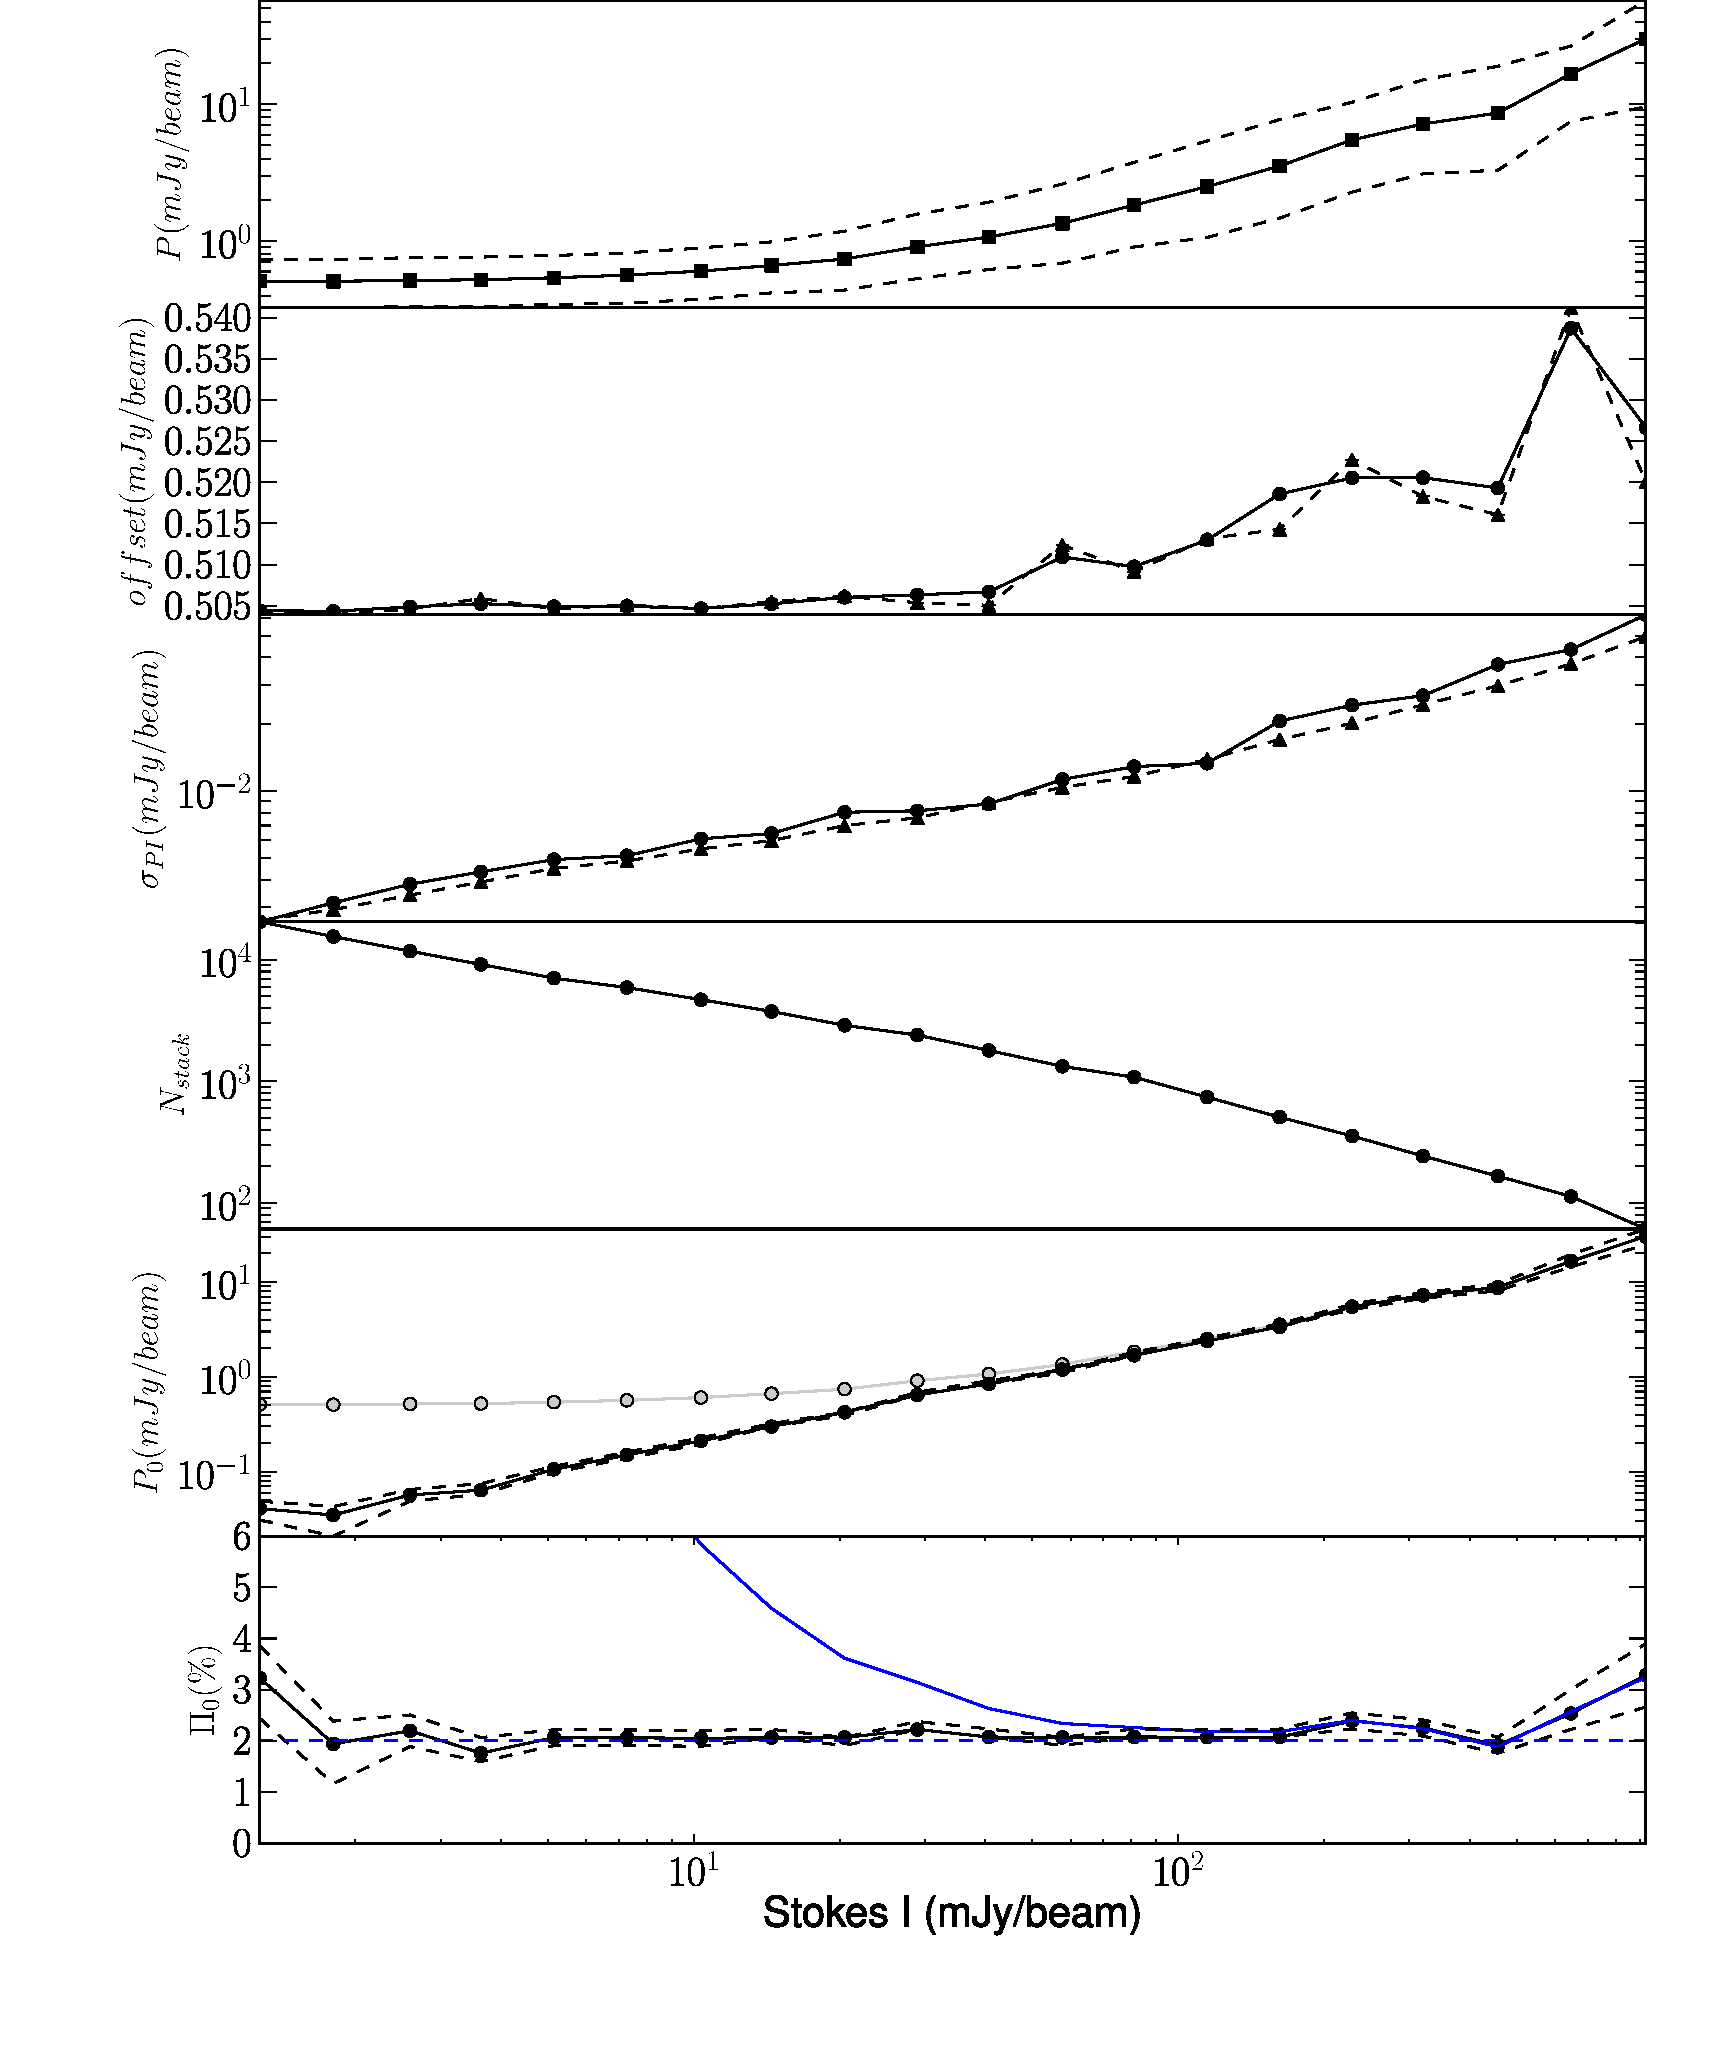
\includegraphics[trim=2cm 0cm 0cm 0cm, clip, scale=0.65]{simulation.eps}\\
\caption[Simulation Stacking Statistics]{Statistics of Simulated NVSS Stack}
\centering
\end{figure}

\section{Usage Example: NVSS Stacking}
\subsection{Setup}
The PASTA suite of tools can be used for determining a percentage 
polarization curve for the NVSS extragalactic sources.  In order to do this,  
4\degree x 4\degree images in Stokes \emph{I}, Stokes \emph{Q}, and PI are 
obtained.  In addition to the two sets of image tiles, a sourcelist containing 
the RA, Dec, and Stokes \emph{I} value of each source is used.  This list 
is split into logarithmic Stokes \emph{I} flux bins, defined as:
$$\mathrm{F_{upper}} = 10^{0.05}\mathrm{F_{lower}}$$
with a minimum flux of 2.000 mJy and a maximum flux of $\approx1$ Jy. The RMS
background of the NVSS is 290 $\mu$Jy in Stokes \emph{Q} and \emph{U}, and 
450 $\mu$Jy in Stokes \emph{I}.  Running at a maximum noise of $2\sigma$ yields
a maximum noise value of 580 $\mu$Jy for the \emph{Q} stack.

\subsection{Stacking Stokes \emph{Q}}
The first stack to be generated is a Stokes \emph{Q} stack.  Our noise 
rejection is done based on the noise in \emph{Q}, as this noise value is what
is used by the modeller to generate an estimate on the true polarization.  In 
order to generate the stacked results, the following command is used:
\begin{center}
\verb!genstack.py -g 8 -m 0.00058 fluxbinlist  list_of_Q_images 30!
\end{center}

This will generate a stack for the given list consisting on stamps 30 pixels 
square pulled from the list of Q images.  Each stamp will have an absolute 
median border value of less than 580 $\mu$Jy, and will have been regridded by a
factor of 8.

\subsection{Stacking Stokes \emph{I} and PI images}
Once a set of Q stacks has been completed, the noise files from each stack are
used to generate \emph{I} and PI stacks.  The command used to generate these
stacks is:

\begin{center}
\verb!genstack.py -n -g 8 noise_fluxbinlist.dat list_of_I_images 30!\\
\verb! genstack.py -n -g 8 noise_fluxbinlist.dat list_of_PI_images 30!
\end{center}
\noindent
This will generate stacks for \emph{I} and PI containing only sources accepted
in the \emph{Q} stack run earlier.

\subsection{Running the Noise Modeller}
Once the stacks have completed running,  the modeller is run on the output.  In
order to generate a set of modelled stacks, the following command was issued
for each \emph{Q} noise file:
\begin{center}
\verb!mk_stat_varp0 noise_fluxbinlist.dat min_flux max_flux step!
\end{center}

The \verb!min_flux, max_flux,! and \verb!step! are the values of the minimum and
maximum true polarized intensity to test, and the step size between them.  
These units were in Jy, as the NVSS images store in units of Jy.  This generates
a series of files, with file names containing the true polarization values used
to generate them.  To obtain the most likely polarization for a given stack,
the median value of the observed polarizations stored in these files was 
compared to the observed stack polarization.  The closest result is the most 
likely true polarization.

\subsection{Analyzing Results}
The resulting stack results can be passed to the modelling software in order to obtain an estimated $P_0$.  The result can be read by \verb!mktable.sh! to generate a plot of the statistics of the NVSS stack.  To do this, simply pass the 
name of the \emph{Q} noise file as an argument to \verb!mktable.sh!:
\begin{center}
\verb!mktable.sh noise_fluxbinlist.dat!
\end{center}
The table shown on the following page is a plot of the resulting statistics 
generated by the stacking process.  The 6 panels, from top to bottom, are 
described as follows:
\begin{enumerate}
	\item Shows the observed PI of the stacked image, with the 
	solid line corresponding to the median polarization, with the two 
	dashed lines corresponding to the upper and lower quartiles of the 
	stack.
	\item Shows the absolute median background levels for the stack (solid 
	line), and the modeller (dashed line).
	\item Shows the RMS value of the stack (solid line), and the modeller 
	(dashed line)
	\item Shows the number of stamps in the stacked image.
	\item Shows the true polarization value (black line), along with the
	16.5\textsuperscript{th} and 83.5\textsuperscript{th} percentile values 
	(dashed lines), and the observed polarization (grey line)
	\item Shows the percentage polarization of a number of values.  The 
	dashed blue line shows a constant 2\% polarization.  The solid blue line
	shows the observed polarization.  The solid black and dashed black lines
	are the most likely true polarization and 16.5\textsuperscript{th} and 
	83.5\textsuperscript{th} percentile values obtained from the modeller.
\end{enumerate}

\begin{figure}[H]
\begin{center}
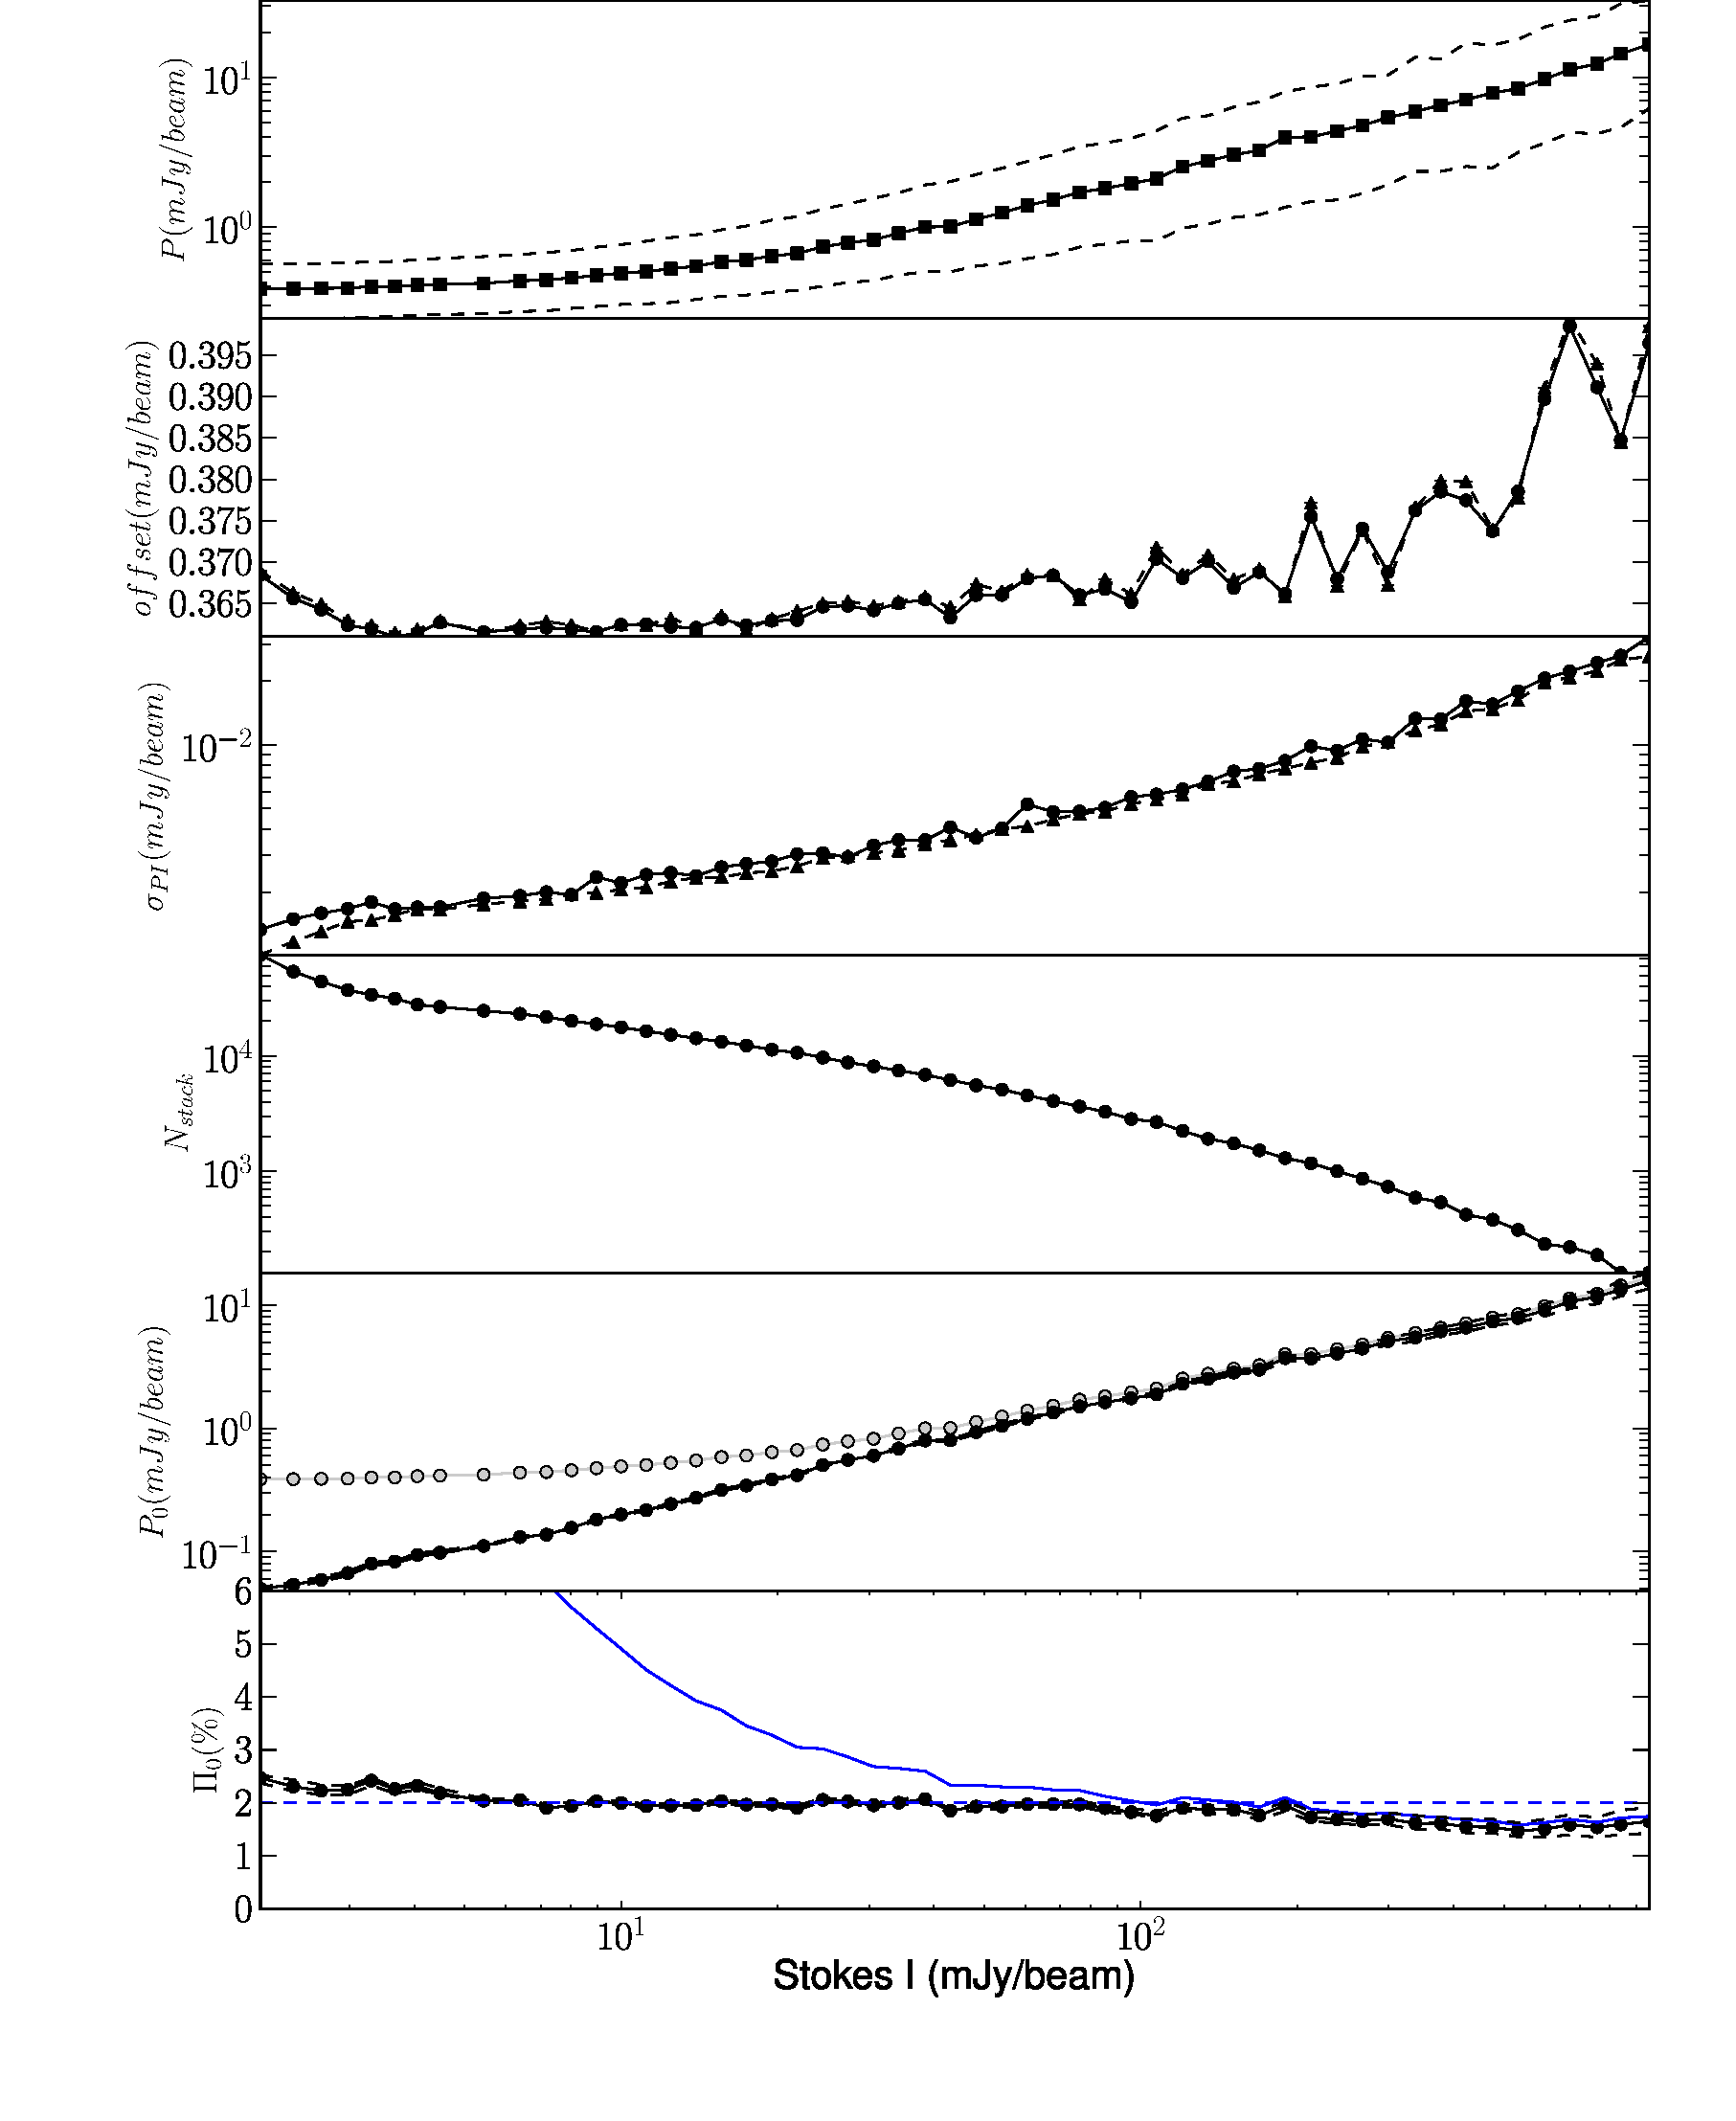
\includegraphics[trim=2cm 0cm 0cm 0cm, clip, scale=0.61]{NVSS.eps}\\
\end{center}
\caption[NVSS Stacking Statistics]{Statistics of NVSS Stacks as a function of 
Stokes \emph{I} Intensity}
\end{figure}


\renewcommand{\refname}{\section{References}}
\begin{thebibliography}{1}
\bibitem{stil2010} The Stacking Paper
\bibitem{NVSS1998}
	Condon, J. J., Cotton, W. D., Greisen, E. W., Yin, Q. F., 
	Perley, R. A., Taylor, G. B., Broderick, J. J.: 1998
	\emph{The Astronomical Journal} {\bf 115} 1693
\bibitem{SandS1985}
	J.F.L Simmons, B.G. Stewart: 1985, 
	\emph{Astronomy and Astrophysics} {\bf 142} 100
\bibitem{BandG2004}
	R. Beck, B.M. Gaensler: 2004
	\emph{New Astronomy Reviews} {\bf 48} 1289
\end{thebibliography}
\end{document}
